\section{Wybrane własności przestrzeni topologicznych i metrycznych}
 
\begin{df}
  Wagą przestrzeni topologicznej $M$ nazwiemy najmniejszą liczbę kardynalną $\kappa$ taką, że istnieje baza $M$ mocy $\kappa$. Piszemy wówczas $\wght M = \kappa$.
\end{df}
 
\begin{lem} \label{lem:base-small}
  Niech $M$ będzie przestrzenią topologiczną o własności $\wght M \geq \aleph_0$. Niech $\mathcal B$ będzie bazą $M$. Wówczas z $\mathcal B$ można wybrać podzbiór $\mathcal B_0$ o mocy nie większej niż waga przestrzeni, tj.:
  \[
    \card \mathcal B_0 \leq \wght M,
  \]
  który jest również bazą.
  \begin{proof}
    Niech $\mathcal D$ będzie bazą $M$ o mocy równej $\wght M$. Niech $D_0 \in \mathcal D$. Wówczas istnieje $\mathcal B_{D_0} \subset \mathcal B$, który sumuje się do $D_0$, tzn. $\bigcup \mathcal B_{D_0} = D_0$. Niech $B \in \mathcal B_{D_0}$. Ten zbiór, z kolei, sumuje się z pewnej podrodziny $\mathcal D_B$ bazy $\mathcal D$. Ale $\card\mathcal D = \wght M$, więc dla $\mathcal D_0 := \{D\ |\ D \in \mathcal D_B, B \in \mathcal B_{D_0}\}$ mamy $\card\mathcal D_0 \leq \wght M$. Dla każdego $D \in \mathcal D_0$ oznaczmy poprzez $B_D$ dowolny nadziór $D$ wpadający w $\mathcal B_{D_0}$. Wówczas $\mathcal G_{D_0} := \{B_D\ |\ D \in \mathcal D_0\}$ jest podzbiorem $\mathcal B$ mocy nie większej niż $\wght M$, który sumuje się do $D_0$.
    
    Niech
    \[
      \mathcal B_0 := \bigcup_{D_0 \in \mathcal D} \mathcal G_{D_0}
    \]
    Zbiór $\mathcal B_0$ podzbiorem $\mathcal B$ mocy nie większej niż $\wght M \cdot \wght M = \wght M$. Co więcej, jeśli $U$ jest zbiorem otwartym, to możemy go wysumować ze zbiorów bazy $\mathcal D$. Ale każdy ze zbiorów $D \in \mathcal{D}$, możemy wysumować z rodziny $\mathcal G_D \subset \mathcal B_0$. W konsekwencji zbiór $U$ daje się wysumować ze zbiorów rodziny $\mathcal B_0$, a więc $\mathcal B_0$ jest szukaną bazą.
  \end{proof}
\end{lem}
 
\begin{fact}
  Powyższy lemat zachodzi również w przypadku $\wght M < \aleph_0$.
  \begin{proof}(szkic)
    Jeśli przestrzeń $M$ ma skończoną bazę, to sama topologia jest skończona, ponieważ każdy zbiór sumuje się ze zbiorów z bazy. Będziemy konstruować bazę minimalną $\mathcal D$. Weźmy zbiory minimalne w tej topologii względem relacji porządku. Takie zbiory muszą należeć do każdej bazy. Następnie usuńmy z topologii wszystkie zbiory, które dają się wysumować ze zbiorów minimalnych. Procedurę kontynuujemy, tzn. z pozostałych zbiorów bierzemy zbiory minimalne według relacji inkluzji - one znowuż muszą należeć do każdej bazy, bo nie dają się wysumować jako nic innego. Wszystkie sumy zbiorów minimalnych usuwamy.
    
    Powyższa procedura zakończy się w skończenie wielu krokach. Z konstrukcji wynika, że ogół zbiorów minimalnych we wszystkich turach stanowi bazę minimalną oraz, że w dowolnej bazie zawarta jest owa baza minimalna. Dlatego też z $\mathcal B$ można wybrać $\mathcal B_0$ o żądanej własności.
  \end{proof}
\end{fact}
 
\begin{df}
  Łańcuchem w zbiorze $M$ nazwiemy uporządkowaną rodzinę $(U_0, \ldots, U_n)$ podzbiorów zbioru $M$ taką, że:
  \[
    \forall i \in n: U_i \cap U_{i+1} \neq \emptyset
  \]
  Zbiory $U_i$ będziemy nazywać ogniwami.
\end{df}
 
\begin{df}
  Niech $M$ będzie przestrzenią toplogiczną, a $\mathcal B$ ustaloną rodziną podzbiorów $M$. Powiemy, że przestrzeń $M$ jest $\mathcal B$-łańcuchowo spójna, jeśli każde dwa punkty $x,y \in M$ można połączyć łańcuchem $(U_0, \ldots, U_n)$ w $\mathcal B$, tj. $x \in U_0$ i $y \in U_n$, a $U_i \in \mathcal B\ \forall i \in n+1$.
\end{df}
 
\begin{lem} \label{lem:chain-connected}
  Niech $M$ będzie spójną przestrzenią topologiczną, a $\mathcal B$ bazą $M$. Wówczas $M$ jest $\mathcal B$-łańcuchowo spójna.
  \begin{proof}
    Dla ułatwienia będziemy mówić łańcuch zamiast $\mathcal B$-łańcuch.
    Jeśli $M = \emptyset$, to lemat jest prawdziwy. Niech $m_0 \in M$. Niech
    \[
      A := \{m \in M\ |\ \mbox{istnieje łańcuch od $m_0$ do $m$}\}
    \]
    Niech $m \in A$.
    Wówczas istnieje łańcuch $(U_0, \ldots, U_n)$ od $m_0$ do $m$.
    Zatem każdy punkt $m' \in U_n$ jest połączony tym samym łańcuchem $(U_0, \ldots, U_n)$ z $m_0$.
    
    \begin{figure}[h!]
      \centering
      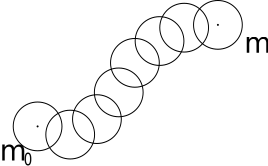
\includegraphics[scale=.5]{img/chain.pdf}
      \caption{Łańcuch od $m_0$ do $m$}
    \end{figure}
    
    Niech $m \in M\setminus A$.
    Weźmy otoczenie $U\in\mathcal B$ punktu $m$. Niech $m'\in U$ i przypuścmy, że $m'\in A$. Zatem istnieje łańcuch $(U_0, \ldots, U_n)$ łączący $m_0$ i $m'$. Ale wtedy $(U_0, \ldots, U_n, U)$ jest łańcuchem łączącym $m_0$ z $m$, czyli $m\in A$, sprzeczność. Zatem $m'\in M\setminus A$.
    
    $A$ jest więc niepustym, bo $m_0 \in A$, zbiorem otwarto-domkniętym. Ze spójności $M$ mamy $A = M$, a więc $M$ jest łańcuchowo spójne.
  \end{proof}
\end{lem}
 
\begin{df}
  Niech $Y$ będzie przestrzenią toplogiczną. Rozmaitością topologiczną modelowaną na $Y$ nazwiemy przestrzeń topologiczną parazwartą $M$ taką, że każdy punkt ma otoczenie homeomorficzne ze zbiorem otwartym w $Y$.
\end{df}
 
\begin{df}
  Atlasem na rozmaitości $M$ nazwiemy rodzinę homeomorfizmów $\{f_c : M \supset U_c \to V_c \subset Y\}_{c \in C}$ pomiędzy zbiorami otwartymi w $M$ i $Y$ -- zwanych również mapami -- taką, że $\bigcup_{c \in C} U_c = M$.
\end{df}
 
\begin{fact} \label{fact:local-metrizability}
  Jeśli $Y$ jest przestrzenią metryczną, to rozmaitość topologiczna $M$ jest również przestrzenią metryczną.
  \begin{proof}(szkic)
    $M$ jest przestrzenią lokalnie metryzowalną, jako przestrzeń lokalnie homeomorficzna z przestrzenią metryzowalną. Z definicji jest też przestrzenią parazwartą. Metryzowalność wynika z twierdzenia o metryzowalności Michaela. [patrz \ref{reference-needed}]
  \end{proof}
\end{fact}
 
\begin{thm}(Twierdzenie A. H. Stone'a)
  \label{thm:stone}
  W dowolne pokrycie otwarte przestrzeni metrycznej można wpisać pokrycie jednocześnie lokalnie skończone i $\sigma$-dyskretne.
  \begin{proof}
    Klasyczny dowód można znaleźć w \cite{ENG}.
  \end{proof}
\end{thm}
 
\begin{cor}
  Niech $Y$ będzie przestrzeią metryczną. Wówczas założenie parazwartości rozmaitości $M$ modelowanej na $Y$ jest równoważne założeniu metryzowalności.
  \begin{proof}
    Z faktu \ref{fact:local-metrizability} mamy, że parazwartość rozmaitości daje jej metryzowalność. Z twierdzenia \ref{thm:stone} wynika, że metryzowalność daje parazwartość.
  \end{proof}
\end{cor}
 
\begin{lem} \label{lem:cl-refinement}
  Niech $M$ będzie parazwartą przestrzenią topologiczną. Wówczas dla każdego pokrycia otwartego $(U_t)_{t \in T}$ przestrzeni $M$ istnieje pokrycie otwarte $(U_t')_{t \in T}$ takie, że $\cl{U_t'}\ \subset U_t\ \forall t \in T$.
  \begin{proof}
    Dowód można znaleźć w \cite{ENG}.
  \end{proof}
\end{lem}
 
\begin{df}
  Pokrycie $(U_t)_{t \in T}$ przestrzeni topologicznej nazwiemy $\star$-skończone, gdy gwiazda każdego elementu tego pokrycia składa się ze skończenie wielu elementów, tj.:
  \[
    \forall t_0 \in T: \card\{t \in T\ |\ U_t \cap U_{t_0} \neq \emptyset\} < \aleph_0
  \]
\end{df}
 
\begin{lem} \label{lem:star-finite}
  Niech $M$ będzie parazwartą przestrzenią topologiczną. Wówczas dla każdego przeliczalnego pokrycia otwartego $M$ istnieje przeliczalne pokrycie otwarte wpisane, $\star$-skończone.
  \begin{proof}
    Dowód można znaleźć w \cite{bp}.
  \end{proof}
\end{lem}
 
\begin{df}
  Powiemy, że rodzina $(U_n)_{n\in\Ni}$ jest uporządkowana w sposób łancuchowo skończony, jeśli nie istnieje nieskończony łańcuch elementów tej rodziny indeksowany silnie rosnącym ciągiem, tzn. nie istnieje $(i_n)_{n\in\Ni}$:
  \[
    i_n < i_{n+1} \wedge U_{i_n} \cap U_{i_{n+1}} \neq \emptyset\ \forall n\in\Ni
  \]
\end{df}
 
\begin{lem} \label{lem:chain-finite-order}
  Każda przeliczalna $\star$-skończona rodzina posiada łańcuchowo skończony porządek.
  \begin{proof}
    Dowód można znaleźć w \cite{bp}.
  \end{proof}
\end{lem}